\documentclass{article}
\usepackage{amsmath,amssymb,amsthm,enumitem} % Some standard math packages.
\usepackage{titling} % Enables \setlength{\droptitle}
\usepackage{parskip} % Cleaner paragraph display
\usepackage[utf8]{inputenc} % Use UTF-8 input encoding instead of default ASCII.
\usepackage{fancyvrb} % Allows Verbatim sections with line numbers and such. Note the capital V.
\usepackage{xcolor} % for text color, e.g. \todo command
\usepackage{ragged2e} % For text alignment environments, e.g. \begin{center}
\usepackage[pdfencoding=auto, psdextra]{hyperref}
\usepackage{graphicx} % For inserting images
\usepackage[a3paper, landscape, textwidth=7in, lmargin=0.75in]{geometry} % 17" wide, 11" tall paper.
\newcommand {\todo}[1] {{\textbf{\color{red}#1}}}
\newcommand {\mq}[1] {\text{`$#1$'}}


%%%
% Section: package configuration
%%%

% Set graphics path, where graphicx will search for images.
\graphicspath{ {./images/} }

\hypersetup{
  colorlinks=true,
  linkcolor=blue!70!black, % Mix 70% blue with 30% black. See package xcolor.
  urlcolor=green!70!black
}

\begin{document}

% Header
\begin{center}
    \Huge
    \textbf{CS 586 Final Project, Part 3}
    
    \Large
    Dylan Laufenberg
    
    \normalsize
    November 30, 2018
\end{center}

\tableofcontents


\section{E/R Diagram}

\textit{Note: I made no changes to the E/R diagram or database schema.}

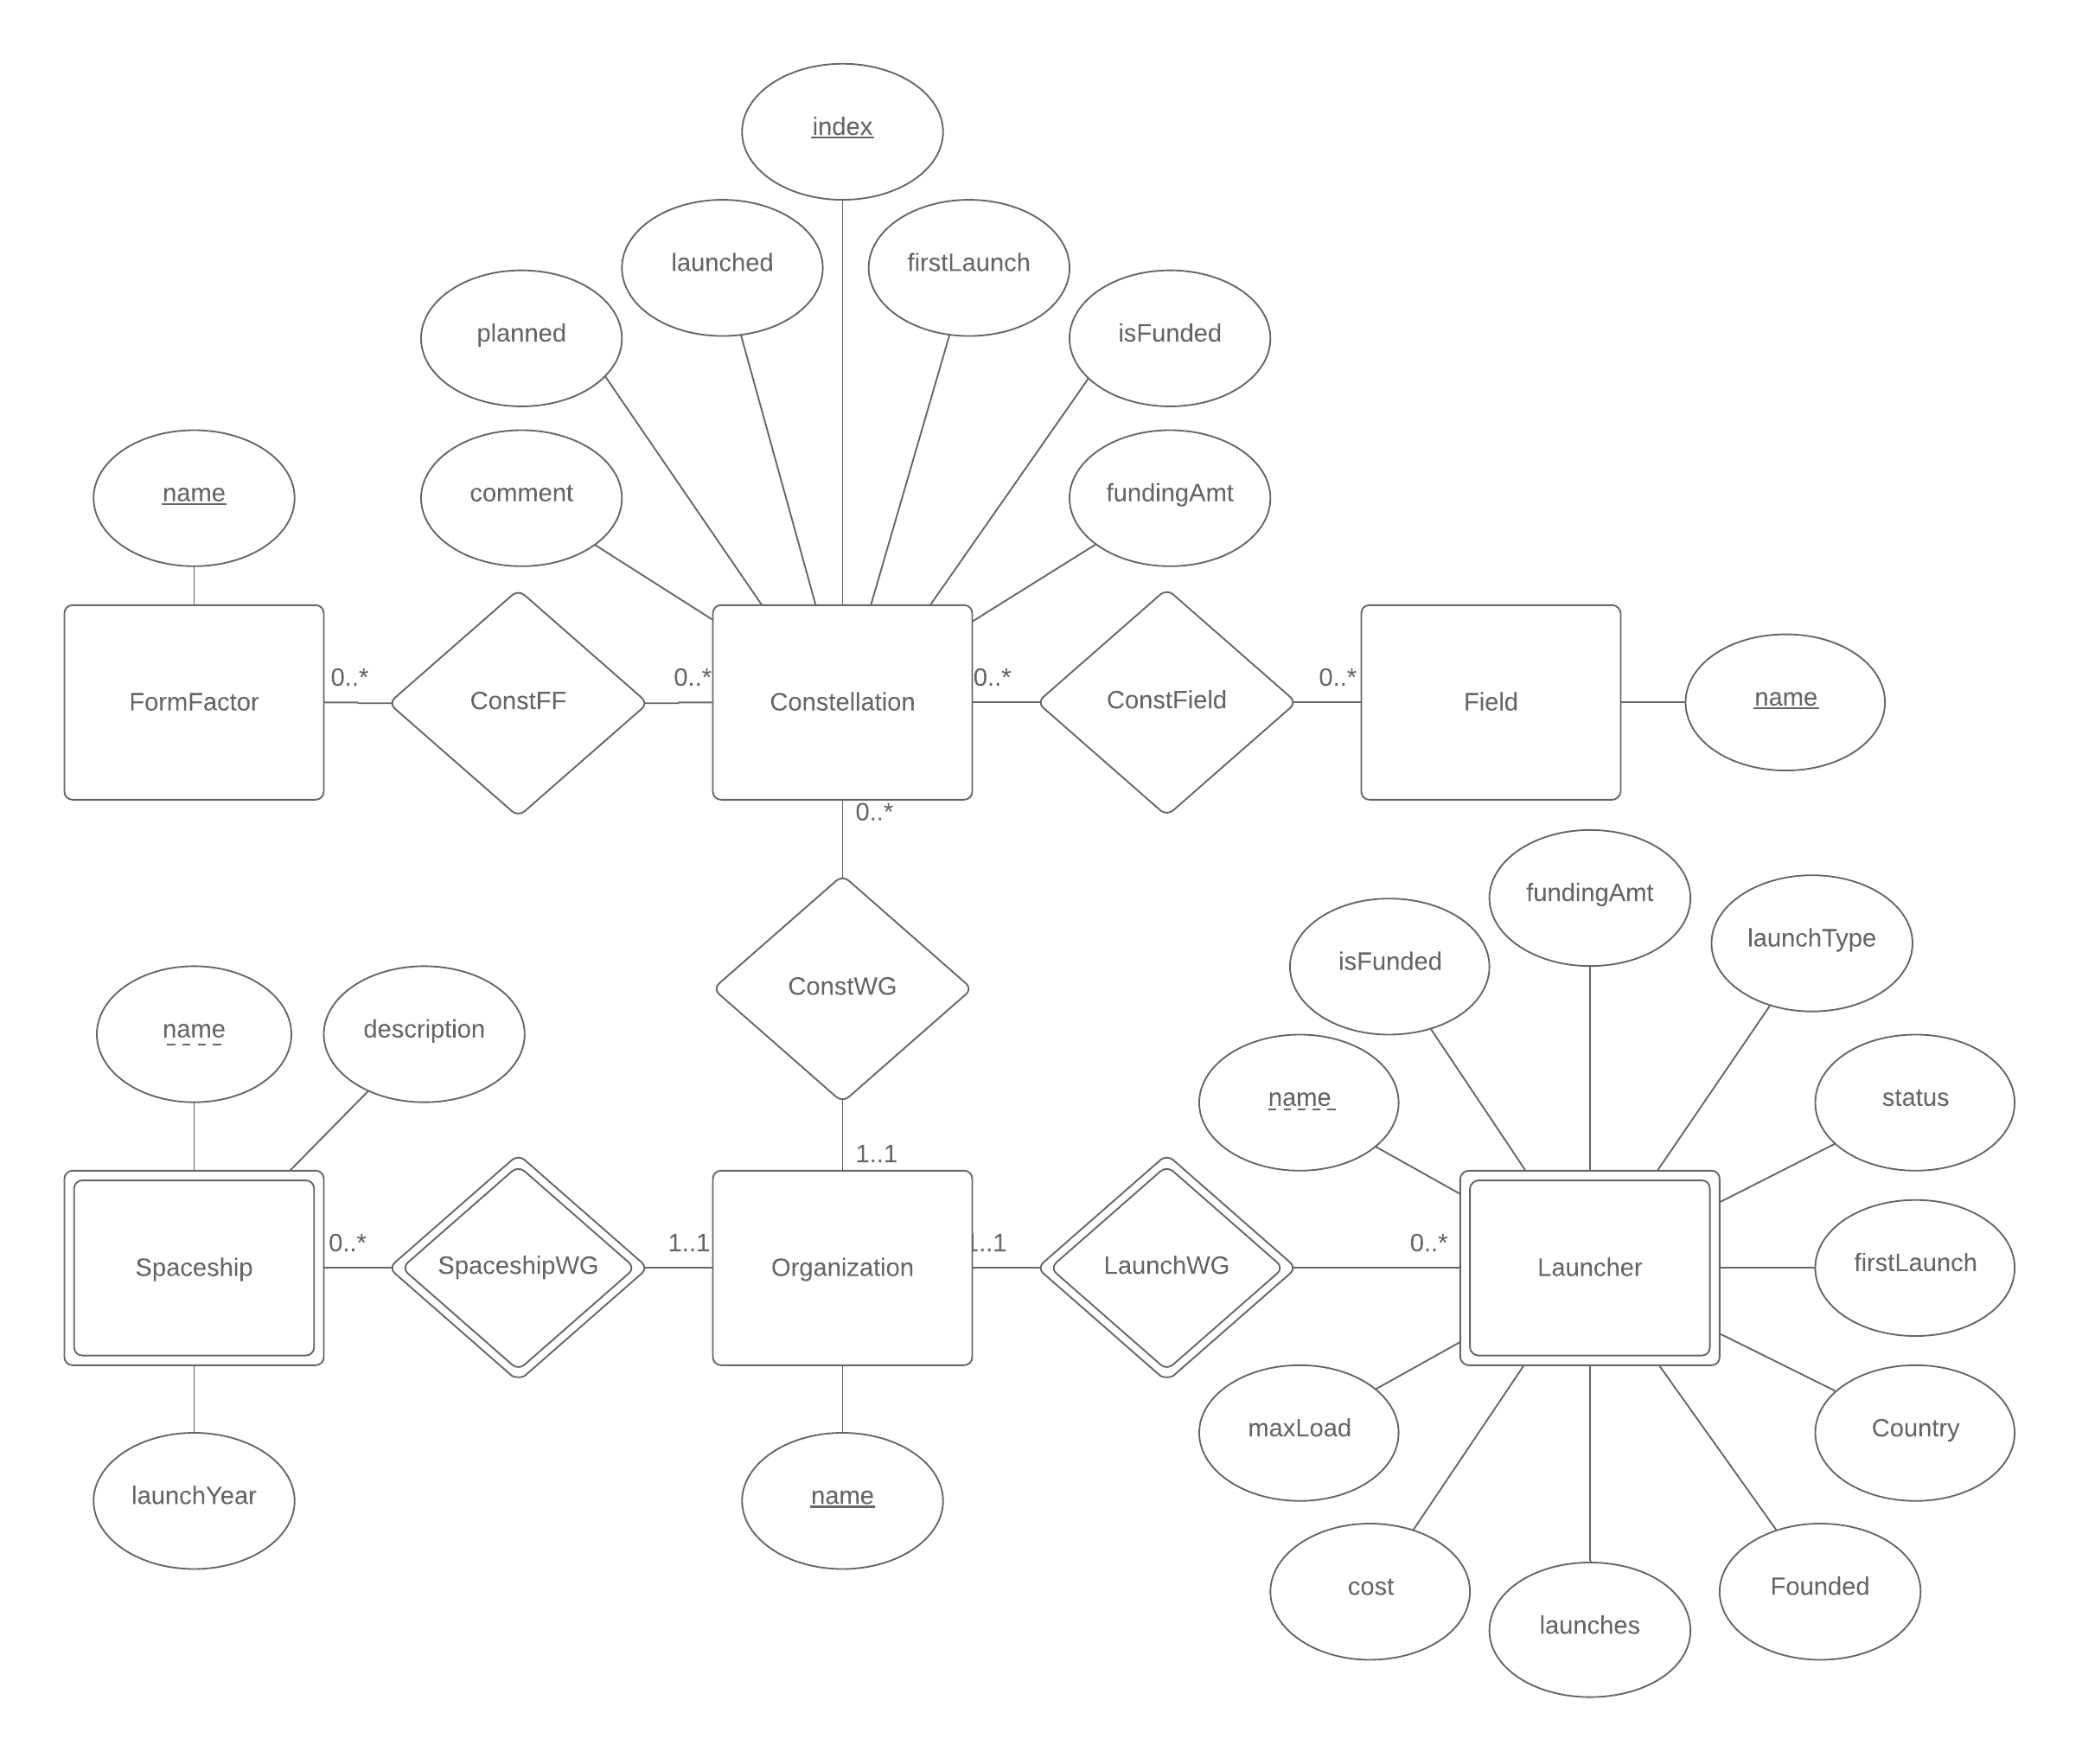
\includegraphics[width=\textwidth]{er-diagram}

\section{CREATE TABLE Statements}

\VerbatimInput{db-contents/create-statements.txt}

\section{Populating the Database}
\href{https://github.com/edev/CS586FinalProject}{View Project on GitHub}

To populate the database, I used a combination of Excel, LibreOffice Calc, Visual Studio Code (VSCode), Vim, and Python 3 (written using Jetbrains PyCharm).

I copied the data from the original source (\href{https://www.newspace.im/index.html}{link}) into multiple sheets in Excel, which, fortunately, preserved most of the cell data properly. I cleaned the data up as much as possible within Excel, saved a .xls document, and exported a tab-separated value (TSV) file with UTF-8 encoding containing just the Constellation table. Next, I wrote a simple \href{https://github.com/edev/CS586FinalProject/blob/master/python/reader/tsvreader.py}{TsvReader} class in Python to give me a line-by-line, iterable reader for TSV files. I attempted to parse and print the data, and Python raised exceptions for unrecognized characters.

Excel didn't show any odd characters at the locations where Python raised exceptions. I opened the .xls and TSV files in LibreOffice Calc to attempt to see if it would show them, but it did not. Next, I opened the TSV file in Vim, to no avail. Back on Windows, VSCode finally showed me diamond question marks for the unrecognized characters and let me replace them with find-replace. (The culprits turned out to be non-breaking spaces in the HTML that Excel didn't handle gracefully, plus some characters in description text that were from highly unusual Chinese character sets.) After this clean-up, Python read and outputted the data correctly. I repeated the VSCode clean-up process for all of the Excel sheets.

With Python able to read the data, I created a simple library of data classes (\href{https://github.com/edev/CS586FinalProject/tree/master/python/dataclass}{link}) to store records in Python and generate SQL output. I wrote a simple, heavily-commented \href{https://github.com/edev/CS586FinalProject/blob/master/python/main.py}{script} to parse each TSV file in turn using TsvReader and the data classes. The script built a list of records for each table, pulling out denormalized information and generating junction table entries as needed. The script wrote a series of SQL files each containing an \texttt{INSERT} statement to populate one table. (For details of what the script does, please see the script itself. The comments should make it quite easy to follow.)

I wrote \texttt{CREATE TABLE} statements by hand and executed them via \texttt{psql}. Next, I ran the generated SQL \texttt{INSERT} statements in an order that would satisfy foreign key dependencies, e.g. I loaded Organization before Constellation/Launcher/Spaceship. I ran \texttt{SELECT} queries to verify that all data appeared to be successfully imported.

\section{Questions}

    % 1
    \subsection{How many different organizations have satellite constellations?}
    \VerbatimInput{questions/1.txt}
    
    % 2
    \subsection{How many satellite constellations does each organization have?}
    \textit{Note: due to the insertion order (and the lack of any ORDER BY clauses), some ordering artifacts will appear in queries, such as all organizations with constellations appearing first due to their order of insertion and the lack of an index on Organization.name.}
    \VerbatimInput{questions/2.txt}
    
    % 3
    \subsection{What is the average number of constellations per organization, excluding organizations that have no constellations?}
    \VerbatimInput{questions/3.txt}
    
    % 4
    \subsection{What organizations have both constellations and upcoming spaceships?}
    \VerbatimInput{questions/4.txt}
    
    % 5
    \subsection{How many organizations have constellations or launchers?}
    \textit{Original: ``What organizations have both constellations and launchers?'' (Changed to add variety, based on grader feedback from Part I of the project.}
    
    \VerbatimInput{questions/5.txt}
    
    % 6
    \subsection{What organizations have launchers but no upcoming spaceships?}
    \textit{Original: ``What organizations have both launchers and upcoming spaceships?'' (Changed to add variety, based on grader feedback from Part I of the project.}
    \VerbatimInput{questions/6.txt}
    
    % 7
    \subsection{What organizations have all 3?}
    \VerbatimInput{questions/7.txt}
    
    % 8
    \subsection{How many constellations use more than 1 form factor?}
    \textit{Note: because constellations do not have names in the original data set, answering this question requires me to make a decision, as the user, about how to identify constellations. I will use the Constellation.index attribute to uniquely identify constellations and include the Constellation.orgName attribute to make the query's results more human-readable. \{index, orgName\} is a superkey, so including orgName will not change the results of the query except to add the orgName column. I also add a count column for easier grading/verification.}
    \VerbatimInput{questions/8.txt}
    
    % 9
    \subsection{What constellations use the most form factors?}
    \textit{Note: The same notes as question 8 apply here as well.}
    \VerbatimInput{questions/9.txt}
    
    % 10
    \subsection{What constellations use only 1 form factor?}
    \textit{Note: The same notes as question 8 apply here as well.}
    \VerbatimInput{questions/10.txt}
    
    % 11
    \subsection{How many projects (constellations, upcoming spaceships, and launchers) first launch each year? (List the number of launches in each year.)}
    \textit{Note: I sort by year even though the question does not ask for it; it just seems like common sense, given the question.}
    \VerbatimInput{questions/11.txt}
    
    % 12
    \subsection{What year saw the most launches (of any kind)?}
    \textit{Note: a vastly simpler query is possible by simply excluding the blank years from question 11 and using LIMIT 1, but in the event of a tie, that query would only display one. This might be valid/expected for some applications, but I use a query that will include any ties in my result.}
    \VerbatimInput{questions/12.txt}
    
    % 13
    \subsection{The launchers listed are in many different statuses (stages of their lifecycles). How many launchers are in each stage/status?}
    \VerbatimInput{questions/13.txt}
    
    % 14
    \subsection{Which launch type is most popular among launchers?}
    \textit{Note: in part I of the project submission, the grader asked, ``Overall, or per launcher?'' To answer this question: each launcher has a launchType field that stores a text value. This question is asking what launchType value is most popular.}
    \VerbatimInput{questions/14.txt}
    
    % 15
    \subsection{Which launch type is most popular among launchers that are currently in development?}
    \VerbatimInput{questions/15.txt}
    
    % 16
    \subsection{How much does the most expensive launcher cost? How much does the least expensive launcher cost? What's the average cost of a launcher?}
    \textit{Original: ``What's the most expensive launcher? What's the least expensive? What's the average?'' Edited for clarity.}
    \VerbatimInput{questions/16.txt}
    
    % 17
    \subsection{How much money has been spent so far on constellations and launchers (ignoring the ones for which we do not have funding numbers)?}
    \VerbatimInput{questions/17.txt}
    
    % 18
    \subsection{How many constellations at least 80\% full (at least 80\% of planned satellites are launched)?}
    \textit{Original: ``How many constellations are full (all planned satellites are launched)?'' Changed according to grader's suggestion.}
    
    \textit{Note: I've opted to include a few additional, relevant fields for easier grading / out of general curiosity. Also, Planet's constellation is indeed at 324/150, according to the original data source (\href{https://www.newspace.im/}{link}). This is not a SQL import error.}
    \VerbatimInput{questions/18.txt}
    
    % 19
    \subsection{How many constellations, launched satellites, and planned satellites pertain to each field?}
    \VerbatimInput{questions/19.txt}
    
    % 20
    \subsection{What constellations have the most planned but unlaunched satellites?}
    \VerbatimInput{questions/20.txt}

\section{Full Listing By Table}

\subsection{Organization}
\VerbatimInput{db-contents/organization.txt}

\subsection{Constellation}
\textit{Note: comment field is truncated to fit within page width.}
\VerbatimInput{db-contents/constellation.txt}

\subsection{ConstFF}
\VerbatimInput{db-contents/constff.txt}

\subsection{FormFactor}
\VerbatimInput{db-contents/formfactor.txt}

\subsection{ConstField}
\VerbatimInput{db-contents/constfield.txt}

\subsection{Field}
\VerbatimInput{db-contents/field.txt}

\subsection{Launcher}
\VerbatimInput{db-contents/launcher.txt}

\subsection{Spaceship}
\VerbatimInput{db-contents/spaceship.txt}

\end{document}